\documentclass[xcolor=dvipsnames,t]{beamer} 

\usepackage{listings} 
\usepackage{color} 
\usepackage{xcolor}  
\usepackage{microtype} 
\usepackage{helvet} 
\usepackage{inconsolata} 
\usepackage[framemethod=TikZ]{mdframed} 
\usepackage{graphicx} 
\usepackage{alltt}
\usepackage{sverb} 
\usepackage{verbatim} 

%\include{ipython-preamble}
\include{mikepsn-preamble} 

\title[Multimodal Virtual Environments]{The Case for Multimodal Virtual
Environments\\ in Multi-Agent Simulations} 

%\subtitle{Designing Virtual Environments for Artificial Intelligence in
%Computational Simulations and Video Games} 

\author[Michael Papasimeon]{Dr Michael Papasimeon \\[0.2in] 
                Workshop on\\ 
                \textbf{Multimodal Human-Agent Interfaces for Virtual Environments} \\[0.2in] 
                Macquarie University\\
                Sydney\\} 
\date{20 November 2014}

\subject{Talks} 

%\usetheme{Rochester} 
%\usetheme{Warsaw} 
%\usetheme{Berkeley} 
%\usetheme[compress]{Berlin} 
%\usetheme{Frankfurt} 
%\usetheme{Darmstadt} 
%\usetheme{Boadilla} 
\usetheme{Madrid} 
%\usetheme{AnnArbor} 
%\usetheme{CambridgeUS} 
%\usetheme{Marburg} 
%\usetheme{Malmoe} 
%\usetheme{Antibes} 
%\usetheme{default} 
%\usecolortheme[named=Red]{structure}
%\usecolortheme{dove} 
\setbeamertemplate{navigation symbols}{}
\setbeamertemplate{blocks}[default]
%\usefonttheme{structurebold} 


\begin{document}

\begin{frame}
    \titlepage
\end{frame} 

\begin{frame}{Context} 

    \begin{block}{Computer Science} 
    Artificial Intelligence and Intelligent Agents 
    \end{block}

    \begin{block}{Software Engineering} 
    Multi-Agent Simulations
    \end{block} 

    \begin{block}{Computational Science} 
    Computational Operations Research
    \end{block} 
\pause
    \begin{exampleblock}{Aim} 
        \begin{itemize}
            \item Authentic, credible and situated computational models of human decision
            making in multi-agent simulations used in computational operations
            research. 
        \end{itemize} 
    \end{exampleblock} 

\end{frame} 

\begin{frame}{Agent-Environment Interaction} 
    Perception-Reasoning-Action Model 
    \begin{center}
        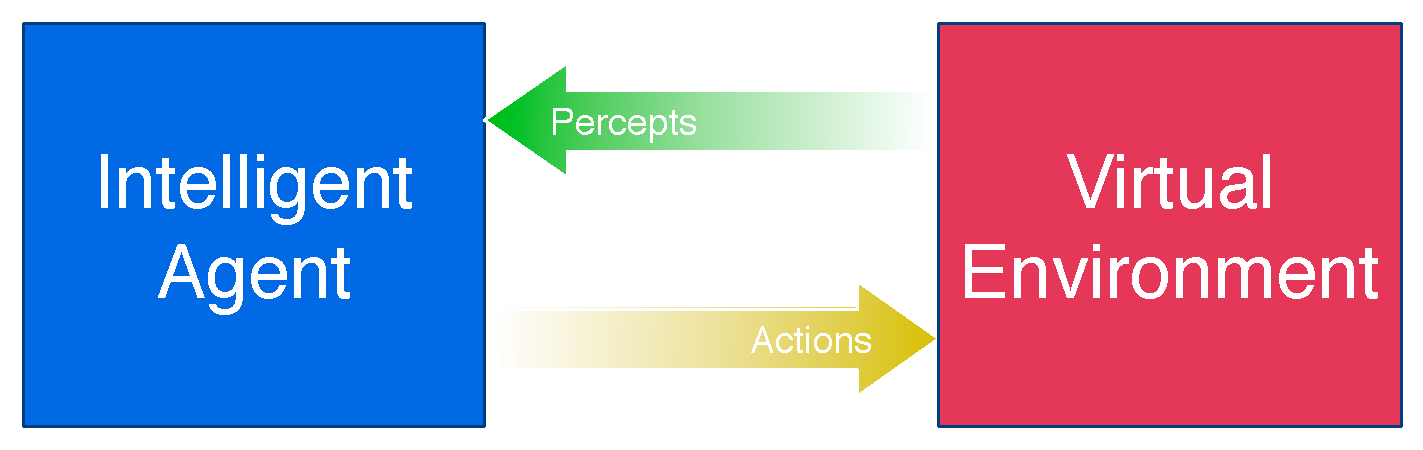
\includegraphics[width=8cm]{agent-env} 
    \end{center} 

    \begin{description}
        \item[Virtual Environment] a dynamic computational representation of a
        world~\footnote{Real, fictitious or abstract world} 
        populated by entities and intelligent agents. 
        \item[Intelligent Agents] an autonomous decision making entity situated
        in virtual environment that can perceive the environment, reason and
        make decisions and take action in the environment.  
    \end{description} 
\end{frame} 



\begin{frame}{Spectrum of Agent-Human Interaction} 
    \begin{center}
        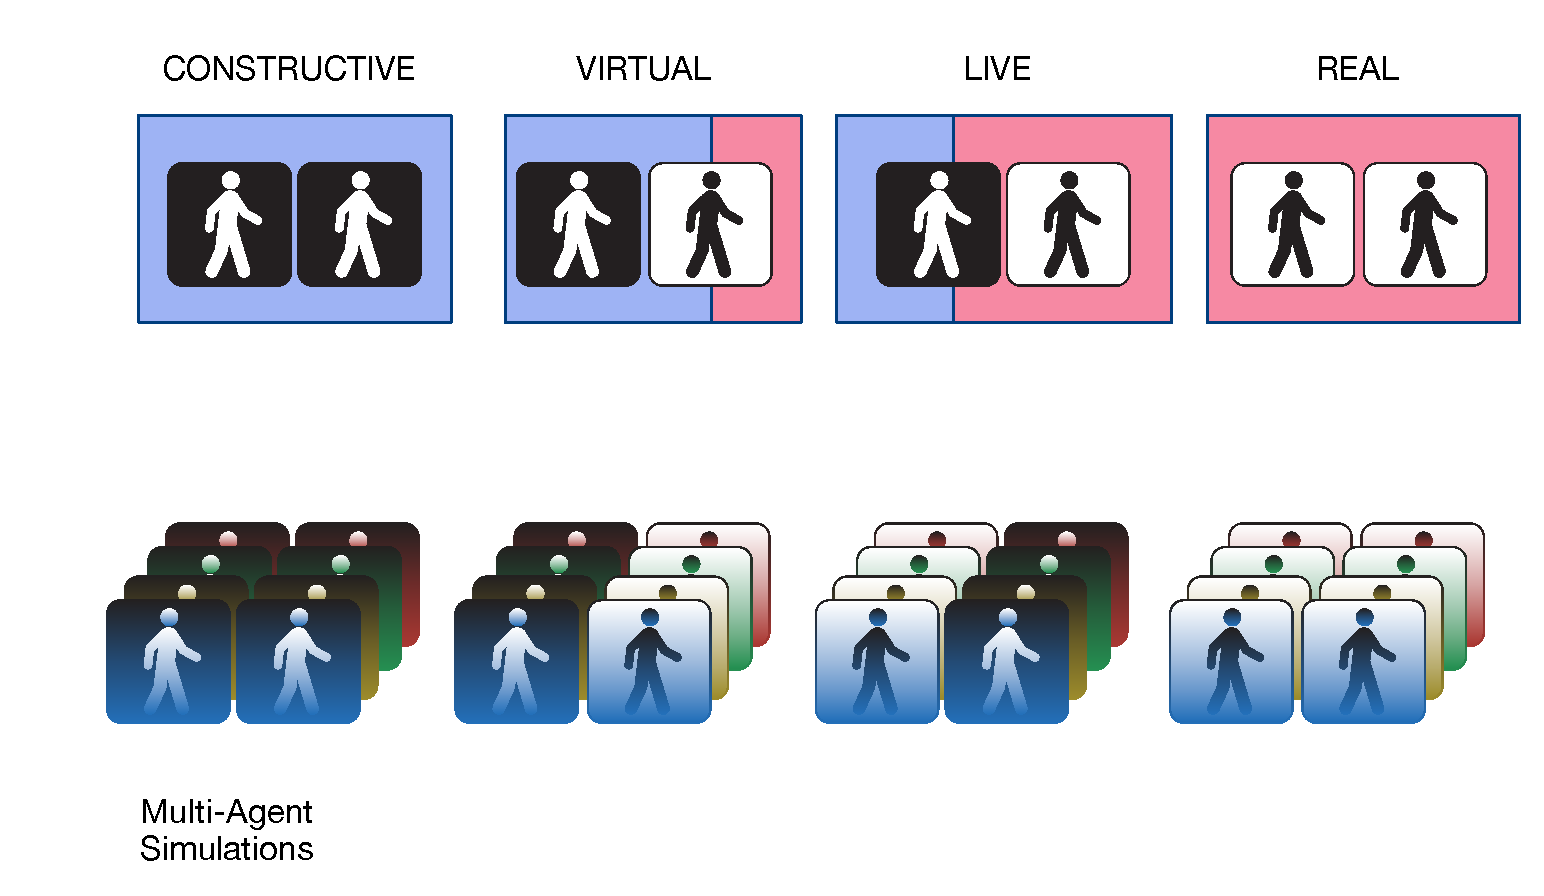
\includegraphics[width=\textwidth]{spectrum} 
    \end{center} 
\end{frame} 

\begin{frame}{Multi-Modal Virtual Environments} 
    \begin{center}
        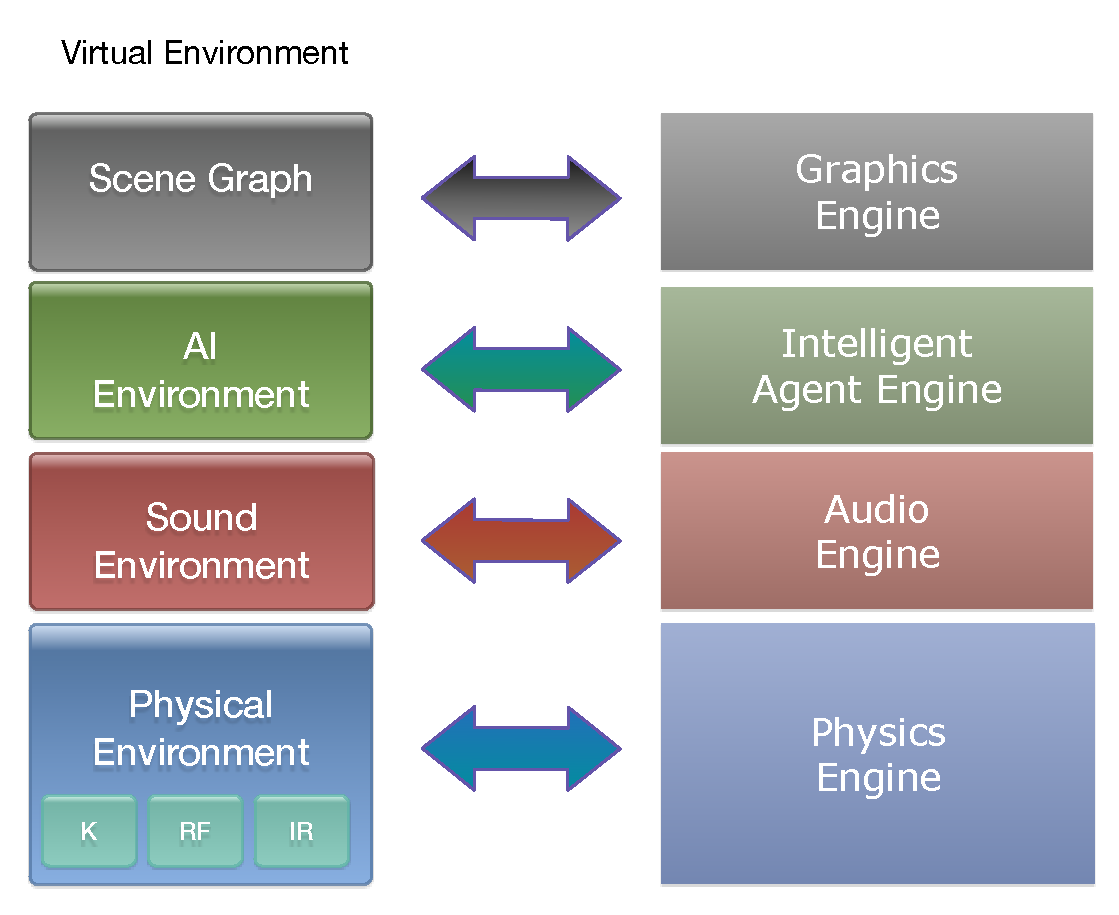
\includegraphics[width=8cm]{multi-modal} 
    \end{center} 
    \tiny See: \emph{The Human-Agent Virtual Environment} Papasimeon, Pearce and Goss. \\
    6th International Conference on Autonomous Agents and Multi-Agent Systems, 2007 
    \normalsize
\end{frame} 

\begin{frame}{Ecological Psychology} 
    The study of how humans and animals interact with the environment they are
    situated in. 

    \begin{block}{Ecology} 
        Ecology = Environment + Humans/Animals + Interaction 
    \end{block} 
\pause
    \begin{block}{Virtual Ecology} 
        Virtual Ecology = Virtual Environment + Intelligent Agents + Interaction 
    \end{block} 
\pause
    \begin{itemize} 
        \item A Multi-Agent Simulation or a Video Game is an example of a virtual ecology. 
        \item Designing one of these systems involves designing a virtual ecology. 
    \end{itemize} 
\end{frame} 

\begin{frame}{Affordance Theory} 
    One of the key ideas in Ecological Psychology is the Theory of Affordances.

    \begin{block}{Affordances} 
        Affordances are the action possibilities an environment provides an agent.
    \end{block} 
\pause
    \begin{block}{J.J. Gibson's Definition} 
        \emph{The affordances of the environment are what it offers the animal, what it
        provides or furnishes, either for good or ill.} 
    \end{block} 
\pause 
    \begin{block}{Direct Perception} 
        Gibson claimed that affordances (action possibilities) are directly perceivable
        by humans and animals in the environment. 
    \end{block} 
\end{frame} 

\begin{frame}{Computing Affordances} 
    \begin{itemize} 
        \item The action possibilities available to an agent depend on many
            different things... not just the physical environment. 
        \item Action possibilities maybe influenced by the social, command,
            electromagnetic, team, network or other abstract environments. 
        \item We want action possibilities that are dynamic, observer
            tailored, relational, intentional/goal oriented, introspective,
            meaningful and context sensitive.~\footnote{\emph{Modelling
                Agent-Environment Interaction in Multi-Agent Simulations with
            Affordances}.  M.  Papasimeon. 2009}
        \item In order to compute affordances (or find the action
            possibilities), our virtual environments have to be
            inherently \emph{multimodal} 
    \end{itemize} 
\end{frame} 

\begin{frame}{Take Home Points...} 
    \begin{itemize} 
        \item Designing situated intelligent agents means we need to consider the 
          agent-environment interaction as an ecology. 
        \item That is we should be talking about... \emph{Designing Virtual Ecologies}
        \item Computational models of affordance (action possibilities) give us a
          closer (more situated link) between agent and environment.
        \item However, in order to determine what actions are possible (what the
          environment affords the agent) the environment needs to be
          \emph{multimodal} 
\end{itemize} 

    \begin{alertblock}{Challenges}
        \begin{itemize}
            \item Non-situated models of agency
            \item Design of Agent-Friendly Virtual Environments
            \item Software Engineering 
            \item Adoption of Ecological Models
        \end{itemize} 
    \end{alertblock} 
\end{frame} 


\end{document} 


